\scanpage{46}
\margin{45}
\figure{
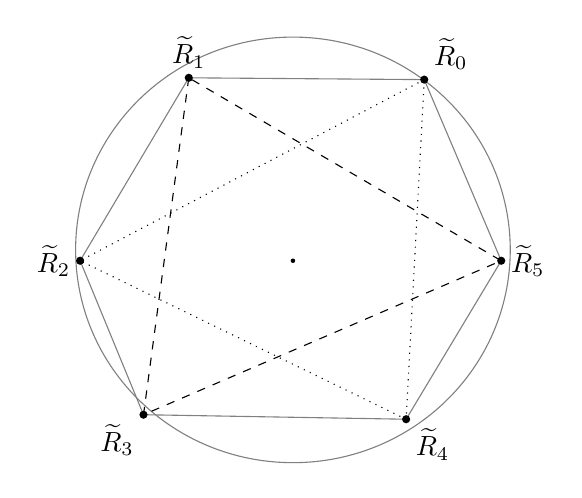
\begin{tikzpicture}[scale=1.15]
\coordinate (r0) at (1.35,2);\coordinate (r1) at (-1.25,2.02);
\coordinate (r2) at (-2.45,0);\coordinate (r3) at (-1.75,-1.7);
\coordinate (r4) at (1.15,-1.75);\coordinate (r5) at (2.2,0);
\draw[gray] (-.1,.12) ellipse (2.4 and 2.35);
\draw[gray] (r0)--(r1)--(r2)--(r3)--(r4)--(r5)--cycle;
\draw[dotted] (r0)--(r2)--(r4)--cycle;
\draw[dashed] (r1)--(r3)--(r5)--cycle;
\fill (-.1,0) circle(.025);
\foreach \p in {r0,r1,r2,r3,r4,r5}{\fill (\p) circle(.045);}
\node[above right] at(r0){$\widetilde R_0$};\node[above] at(r1){$\widetilde R_1$};
\node[left] at(r2){$\widetilde R_2$};\node[below left] at(r3){$\widetilde R_3$};
\node[below right] at(r4){$\widetilde R_4$};\node[right] at(r5){$\widetilde R_5$};
\end{tikzpicture}}
On s'intéresse au \unsure{complexifié} $V_{\mathbb C}$, et à la droite
projective complexe
\deleted{$\Sigma_{\widetilde{\unsure{I|J}}}=$}
\[
(10)\qquad\Sigma_{\widetilde{\unsure{I|J}}}(\mathbb C)
=\Sigma_{\widetilde{\unsure{I|J}}}=\Sigma
=\mathbb P(V_{\mathbb C})
=V_{\mathbb C}^*/\mathbb C^*,
\]
\deleted{les} sur laquelle $D$ opère, le noyau de cette opération étant le centre
$\{1,a_0\}$ i.e. $D$ opère par l'intermédiaire de
\[
(11)\qquad D'=D/\{1,a_0\}
\]
(isom. au groupe diédral $D_n$). On désigne par $R_i\in\Sigma$
l'image de $\widetilde R_i$ dans $\Sigma$, de sorte qu'on aura
\[
(12)\qquad R_i=R_{a_0(i)},
\]
En fait l'ens des $R_i$ est indexé de façon naturelle par l'ens quotient
\[
(13)\qquad\unsure{I|J}=\widetilde{\unsure{I|J}}/\{1,a_0\}.
\]

\margin{\uline{NB} $(\Sigma,\unsure{I|J}\subset\Sigma)$ étant donnés
($\Sigma$ comme droite projective complexe, ou comme sphère conforme orientée\ldots)
on a \unsure{équivalemment} un torseur sous $D_n$ $(\ne D_m!)$
\unsure{étant donné}, on peut en déduire $(V,\widetilde{\unsure{I|J}})$
à isom \unsure{non can.} près (i.e. un torseur sous $D_m$), mais seulement
modulo twist par $\{\pm1\}$-torseur\ldots On peut lever l'ambiguïté en imposant
une structure suppl. sur $\widetilde{\unsure{I|J}}$, à savoir la donnée
d'un élément de $\widetilde{\unsure{I|J}}/(D^+)^2$ i.e. de l'un
des deux $n$-gônes dans le $2n$-gône $\widetilde{\unsure{I|J}}$
\unsure{est stable par} $\unsure{C}$ \unsure{pour les ``positifs''}\ldots}
